% LTeX: enabled=false
\documentclass[11pt,a4paper,twoside]{book}
\linespread{1.3}

\usepackage[main=english,polish]{babel}

\usepackage[T1]{fontenc}
\usepackage[utf8]{inputenc}
% \usepackage[sfdefault,scaled=.95]{FiraSans}

\usepackage[lf]{Baskervaldx} % lining figures
\usepackage[bigdelims,vvarbb]{newtxmath} % math italic letters from nimbus Roman
\usepackage[cal=boondoxo]{mathalfa} % mathcal from STIX, unslanted a bit
\renewcommand*\oldstylenums[1]{\textosf{#1}}

\usepackage[table]{xcolor}
\definecolor{plum}{RGB}{150,95,119}
\definecolor{grafit}{RGB}{60,60,60}

\usepackage{amsmath,amsfonts}
% \usepackage{icomma}
\usepackage{textcomp}
\usepackage{gensymb}

\usepackage{graphicx}

\usepackage[left=3cm,right=2cm,top=2.5cm,bottom=2.5cm]{geometry}

\usepackage{fancyhdr}
\pagestyle{fancy}
\renewcommand{\headrulewidth}{0pt}
\renewcommand{\footrulewidth}{1.5pt}
\renewcommand{\footrule}{{\color{plum}%
			\vskip-\footruleskip\vskip-\footrulewidth
			\hrule width\headwidth height\footrulewidth\vskip\footruleskip}}

\fancyhead{}
\cfoot{}
\fancyfoot[LE, RO]{\thepage}

\renewcommand\labelitemi{\color{plum}{\tiny$\blacksquare$}}
\renewcommand\labelitemii{\color{plum}{\tiny$\square$}}
\renewcommand\labelitemiii{\color{plum}{\tiny$\bullet$}}

\usepackage{enumitem}
\setlist[itemize]{noitemsep, topsep=0pt, leftmargin=1cm, itemindent=0cm}

\usepackage{nowidow}
\widowpenalty=10000
\clubpenalty=10000
\brokenpenalty 10000
\sloppy

\usepackage[skip=4pt,indent=0cm,parfill=0pt]{parskip}

\usepackage{array}
\usepackage{multicol}
\usepackage{multirow}
\renewcommand*{\figurename}{Fig.}
\renewcommand*{\tablename}{Tab.}
\setlength{\arrayrulewidth}{1pt}
\arrayrulecolor{plum}
\renewcommand\thefootnote{\textcolor{plum}{\arabic{footnote}}}
\usepackage[font={footnotesize},justification=centerlast]{caption}
\numberwithin{equation}{chapter}
\newcolumntype{M}[1]{>{\centering\arraybackslash}m{#1}}
\usepackage{subfig}

\usepackage{lipsum}

\let\lll=\relax

\usepackage[inkscapelatex=false]{svg}
\usepackage[version=4]{mhchem}
\usepackage{braket}
\usepackage{listings}

\setlength{\jot}{20pt}
\setlength{\parskip}{1em}

\raggedbottom
\renewcommand{\arraystretch}{1.4}

\usepackage{catchfile}
\newcommand{\getenv}[2][]{%
  \CatchFileEdef{\temp}{"|kpsewhich --var-value #2"}{\endlinechar=-1}%
  \if\relax\detokenize{#1}\relax\temp\else\let#1\temp\fi}

\getenv[\INDEX]{INDEX}

\newcommand{\probP}{\text{I\kern-0.15em P}}
\newcommand{\todo}[1]{\textcolor{red}{TODO: #1}}
\newcommand{\thesistitle}{Influence of the reconstruction efficiency on the angular correlation functions in Run 3 software in ALICE.}
\newcommand{\thesistitlepl}{\begin{otherlanguage}{polish}
    Wpływ wydajności rekonstrukcji śladów cząstek na kątowe funkcje korelacyjne w oprogramowaniu Run 3 w eksperymencie ALICE.
\end{otherlanguage}}

\usepackage{hyperref}
\hypersetup{
	pdftitle = {\thesistitle},
	pdfauthor = {Dawid Karpiński},
	colorlinks,
	linktoc=page,
	linkcolor=plum,
	citecolor=plum,
	filecolor=plum,
	urlcolor=plum
}


\begin{document}
\pagestyle{empty}

\begin{titlepage}
    \begin{minipage}{\textwidth}
        \begin{center}
            
\includegraphics[scale=0.2]{img/WF_ENG} \\
            \vspace{1.5cm}
            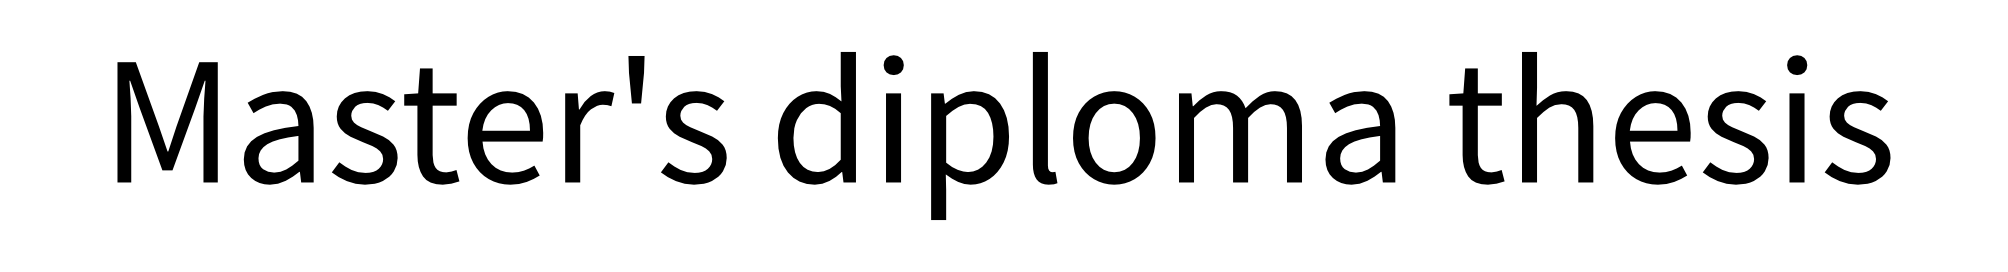
\includegraphics[width=0.7\textwidth]{img/mgr_en}
        \end{center}
    \end{minipage}

    \vspace{1.5cm}

    \begin{minipage}{\textwidth}
        \begin{center}
            {\large in the field of study Fizyka Techniczna \\
                and specialization EDMI}
        \end{center}
    \end{minipage}

    \vspace{1.5cm}

    \begin{minipage}{\textwidth}
        \begin{center}
            {\LARGE \thesistitle}
            \vspace{0.5cm}\\
            {\large thesis number according to Faculty's thesis evidence: \{\todo{number}\}}
        \end{center}
    \end{minipage}

    \vspace{1.5cm}

    \begin{minipage}{\textwidth}
        \begin{center}
            {\LARGE Dawid Karpiński}
            \vspace{0.5cm}\\
            {\large student record book number: \INDEX}
        \end{center}
    \end{minipage}

    \vspace{1.5cm}

    \begin{minipage}{\textwidth}
        \begin{center}
            {\large supervisor: \\
                dr hab. inż. Małgorzata Janik}\\
            \vspace{0.5cm}
            {\large second supervisor: \\
                dr hab. inż. Łukasz Graczyk}
        \end{center}
    \end{minipage}%

    \vfill

    \begin{minipage}[b]{\textwidth}
        \begin{center}
            {\large WARSAW \the\year{}}
        \end{center}
    \end{minipage}
\end{titlepage}

% LTeX: enabled=true

\newpage
\mbox{ }

\newpage
{\Large Abstract}

{\color{plum}\rule[1pt]{\textwidth}{2pt}}

\textbf{Thesis title:} \thesistitle

\todo{abstract}

\vspace{0.025\textheight}
\textit{Keywords}\\
\textit{\todo{keywords}}

\vfill

\begin{multicols}{2}
    \begin{flushleft}
        supervisor's signature
    \end{flushleft}
    \begin{flushright}
        student's signature
    \end{flushright}
\end{multicols}

\newpage
\mbox{ }

\newpage
\begin{otherlanguage}{polish}
    {\Large Streszczenie}

    {\color{plum}\rule[1pt]{\textwidth}{2pt}}

    \textbf{Tytuł pracy:} \thesistitlepl

    \todo{abstract pl}

    \vspace{0.025\textheight}
    \textit{Słowa kluczowe:}\\
    \textit{\todo{klucz}}

    \vfill

    \begin{multicols}{2}
        \begin{flushleft}
            podpis opiekuna naukowego
        \end{flushleft}
        \begin{flushright}
            podpis studenta
        \end{flushright}
    \end{multicols}
\end{otherlanguage}

\newpage
\mbox{ }

\tableofcontents
\addtocontents{toc}{\protect\thispagestyle{empty}}
\pagestyle{empty}

\chapter{Introduction}
\pagestyle{fancy}

\section{LHC and Run 3}

The \textbf{Large Hadron Collider} (LHC), located at the European Organization for Nuclear Research (CERN) near Geneva, Switzerland, stands as the world's largest particle accelerator. Created in 2008, it accelerates and collides particles, primarily protons and heavy ions (e.g., lead). These collisions produce a variety of subatomic particles, allowing us to test our predictions of the Standard Model and search for new phenomena beyond it.

The collider has completed two successful periods of data collection, the first Run 1 (2010--2013), and the other Run 2 (2015--2018). The current operational phase, \textbf{Run 3}, began in 2022 following the second, long shutdown (LS2) \cite{lhc-upgrade}. After the upgrades, the LHC now features proton-proton collisions at a center-of-mass energy of 13.6 [TeV], an increase from the 13 [TeV] utilized in Run 2. This higher energy helps in further studies and improves measurement precision and analysis statistics.

\section{The ALICE experiment}

The acronym ALICE stands for \textbf{A Large Ion Collider Experiment}, one of four major experiments at the LHC. The detector enables to study the quark-gluon plasma (QGP), a state with conditions resembling those a few millionths of a second after the Big Bang, before quarks and gluons combined to form protons and neutrons. Heavy ion nucleus-nucleus collisions can produce such a state. In the case of ALICE, the main focus lies on lead-lead (Pb-Pb) collisions \cite{alice-cern}. The experiment also includes proton-nucleus collisions, as well as analysis of proton-proton collisions as a reference data.


\section{Two-particle angular correlation function}

The main work in this thesis based on $\Delta\eta\Delta\varphi$ particle correlations, that come from proton-proton collision data collected from the ALICE experiment.

\subsection{Pseudorapidity and azimuthal angle}

Once constructs the correlation function using two quantities: pseudorapidity, $\eta$, and azimuthal angle, $\phi$. Both represent different angles in the detector space.

First, the pseudorapidity, $\eta$, relates to the angle between the particle momentum $p$ and the beam axis as such:

\begin{equation}
    \eta = -\ln\left[\tan\left(\frac{\theta}{2}\right)\right]
\end{equation}.

\section{Correction procedure}

\todo{transverse momentum, mc reco, mc truth, detection}

\section{Reconstruction efficiency}

\todo{angles, coordinate system}

\section{Framework — O2 and O2Physics}

\cite{alice-o2}

\section{CCDB}

\bibliography{bib}
\bibliographystyle{unsrt}

\listoffigures
\listoftables

\appendix

\end{document}
